\documentclass[a4paper,10pt]{article}
\usepackage{inputenc}

\usepackage[left=2.5cm,right=2.5cm,top=2cm,bottom=2cm]{geometry}
\usepackage{amsmath,amsfonts,amssymb}
\usepackage{graphicx}
\usepackage[colorlinks=true,linkcolor=blue,urlcolor=blue,citecolor=blue]{hyperref}
\usepackage{color}
\usepackage{listings}

%opening
\title{Skippy Device Server \\
\large sources version 1.5.3-alpha1}
\author{Sergi Blanch-Torn\'e\\\small{Controls Software Engineer - Alba Synchrotron}\\{\tt \small{sblanch@cells.es}}}

\newcommand{\todo}[1]{\texttt{\color{red}TODO:} ``\emph{#1}''}
\newcommand{\fixme}[1]{\texttt{\color{red}FIXME:} ``\emph{#1}''}
\newcommand{\ok}[1]{``#1'' [\texttt{\color{green}OK}]}

\setcounter{secnumdepth}{5}

\begin{document}

\maketitle

\begin{abstract}
Following the \href{https://en.wikipedia.org/wiki/Standard_Commands_for_Programmable_Instruments}{wikipedia}'s definition:  the \texttt{SCPI} ``\emph{defines a standard for syntax and commands to use in controlling programmable test and measurement devices}''. Many scientific instrumentation uses this schema for the configuration and operation of the instrument's purpose.

Since 2007, the \texttt{Alba} Synchrotron has developed a set of \href{http://tango.controls.org}{\texttt{tango} Device Servers} to access instruments that provides this protocol. Development experience has guided us until this \texttt{Skippy} device server. In parallel, due to our own needs over \emph{in-house} development of instrumentation, it has been developed also a \texttt{python} module that provides some of our instruments this interface to the upper layers, called \href{https://github.com/srgblnch/python-scpilib}{python-scpilib}.

The original development of a \texttt{tango} Device Server provides only access from this Distributed Control System (DCS), but it is also good to provide a simple python access in between the instrument and the Control System.

Then with this two developments together, the \texttt{scpilib} and the \texttt{skippy}, the circle has been closed supporting all the points of view over this protocol.

%\texttt{Alba} has used an specific Device Server, under the name \emph{PyVisaInstrWrapper}, to communicate with instruments like scopes, radio frequency generators, arbitrary signal generators and spectrum analyser. This device was an extension from the original \emph{PyScope}, becoming it one of the internal device classes. Before that, there was a \texttt{C++} device server called \emph{TekDPO7000}. This is a long background on this protocol that helps to provide many improvements to this Device Server. %By the way it has start showing certain limitations that may advice bounds of the design. But how this has been developed allows a \emph{refactoring} of the internalities to save those constrains.

%Recent development has requested a \texttt{python} module to provide an \emph{in-house} instrument developed (an electrometer), the result of this becomes the \href{https://github.com/srgblnch/python-scpilib}{python-scpilib}. Those two things together closes a circle on the \texttt{SCPI} providing the instruments the feature to support this protocol as well as provide a way that from \texttt{tango} (or even simply from \texttt{python}) access to this kind of intrument.
\end{abstract}

\tableofcontents

\section{Introduction}

The \texttt{Alba} Synchrotron has collected some experience controlling instruments that supports the \texttt{SCPI} protocol from one or many of the interfaces. Previous to this \texttt{skippy Device Server} we have implemented the \emph{PyVisaInstrWrapper}, that uses lower level \texttt{tango} devices (like it is the \emph{PyVisa} or the \emph{Serial}, to connect to instrument like \emph{oscilloscopes}, \emph{radio frequency generators}, \emph{signal and function generators} and even \emph{spectrum analyzers}.

The \emph{Wrapper} was in fact a generalization of an even previous \emph{PyScope} that was confined to be one of the Device Classes supported. Even before that, there is the first of our instrument control, made in \texttt{C++}, that was only controlling one series of Tektronix scopes. The name \emph{TekDPO7000} says everything.

\section{Design}

The main user case of this project is to access the instruments from \texttt{tango} control system. The design starts from this very above view. A distributed system agent (aka \texttt{device}) in charge of promoting information of a single instrument to the control system has an state machine, common for all kind of instrument below. It normalizes in a common upper view of what would be down there.

But this \texttt{device} does not have the functionalities implemented within itself, the project provides a \texttt{python} module with a main class (called \texttt{Skippy} as one can expect) that in the constructor the \texttt{device} properties are setup to then have a pure python interface to the instrument. This has been made to allow future uses without a \texttt{tango device} (but having a dependency on \texttt{PyTango}) or, and the important case, to migrate the \texttt{device server} code to the \href{http://www.esrf.eu/computing/cs/tango/pytango/v816/server_api/server.html}{High level server API}.

%The main restriction that the \emph{PyVisaInstrWrapper} shows is the dependency on the \emph{PyVisa} subdevice to manage the communications with the instrument. The main issue was the impossibility to define alternatives to the subdevice. Also the growing number of query commands to the instrument has reach the limit of the basic design.

\subsection{Machine state}

When a device of an instance of the \texttt{Skippy} device server is launched, the first state it has is \texttt{INIT}\footnote{There is even a previous state, when it has not been initialised, called \texttt{UNKNOWN}. But immediately in the \texttt{tango device} construction it is set to \texttt{INIT}.}, on the left side of the picture \ref{fig:stateMachine}. When all the internal elements are well initialised, then it changes its state to \texttt{OFF}. At this state, the device has an internal object with the responsibility of the communications with an instrument (but no communication has been started).

Then, if the configuration properties do not say the contrary (details about them will be extended in section \ref{sec:devProp}), the device will try to establish communication with the instrument. This is reported with the state change to \texttt{STANDBY}. The instrument will receive a request to identify itself, and the answer will allow the device to know which instructions set is necessary to talk further with the instrument.

Again, and still the flow is controlled by the configuration properties, the device create the specific set of (dynamic) attributes for the identified instrument. Reporting this succeed with a state change to \texttt{ON}. If there are attributes to have their value monitored and pushing events, and for the last time, the configuration properties will allow or inhibit the next state change, the \emph{Start()} process will be launched to have an specific thread in charge of this monitoring. This state corresponds with \texttt{RUNNING} state, and more details will be explained in \ref{sec:monitor}.

The figure \ref{fig:stateMachine} show other state-change transition, the edges, with the command name that produces the change. In any case, if something goes wrong, its state will decay to \texttt{FAULT}. To recover from fault, the \emph{Init()} command should be called, apart from cases where the device itself can recover the situation to then do the necessary steps to recover normal operation.

\begin{figure}[h]
    \centering{
         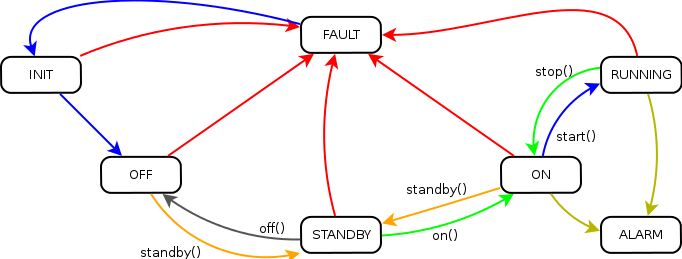
\includegraphics[width=0.75\textwidth]{StateMachine.png}
         \caption{State machine diagram of the Device in the Skippy Device Server} \label{fig:stateMachine}
    }
\end{figure}

There are two more states that the \texttt{device} may report sporadically. When the queries to the instrument takes longer than expected, then the state will be reported as \texttt{ALARM} until the access to the instrument goes back to a normal timing. When this happens the \texttt{device} would try to reduce the load of the instrument by reducing the frequency of queries send to the instrument or the number of queries sent in parallel.

The last of the states is the \texttt{DISABLE}. One of the internal features of this \texttt{device} is to check periodically if the instrument is still available. This is specially important to report a communications fault when the instrument has been shutdown, as well as to recover a communications glitch. \todo{More details about that in section \ref{sec:watchdog} about the \texttt{WatchDog}}.

\subsection{Device as an Object}

As \texttt{Tango} is an \emph{Object oriented} (OO paradigm) DCS, each of the agents have a set of construction parameters, what is called \texttt{Properties} (section \ref{sec:devProp}. Once the \emph{object/agent} is build in the system, it offers a set of \texttt{Attribute} (section \ref{sec:devAttrs}) and \texttt{Commands} (the \emph{methods} in the OO paradigm, section \ref{sec:devCmds}).

\subsubsection{Device Properties}\label{sec:devProp}

\begin{itemize}
    \item {\tt Instrument}: mandatory property to configure the instrument that will be introduced to the distributed system via the device.
    \begin{itemize}
        \item If the content string is a host name, use sockets to communicate with the instrument
        \item If the content string is a device name if the class of this subdevice is \texttt{PyVisa} or even \texttt{[Py]Serial}, it will be used as a bridge to the instrument.
        \item If the content string is a serial line file descriptor (for example a \texttt{/dev/ttyS}\emph{n} or a \texttt{/dev/ttyr}\emph{NN}), it will be the way the instrument will be accessed.
        \item else, decay to fault state with the appropriate status message
    \end{itemize}
    \item {\tt Port}: optional property to specify a port, in the socket communication, when it should be different than the default 5025.
    \item {\tt SerialBaudrate}, {\tt SerialBytesize}, {\tt SerialParity}, {\tt SerialStopbits}, {\tt SerialTimeout},\\ {\tt SerialXonXoff}: optional properties to define the serial line communications when the instrument is accessed by a serial line in the machine where it runs.
    \item {\tt NumChannels}: optional property to define, in case the instrument has channels, the number of them available.
    \item {\tt NumFunctions}: optional property to define, in case the instrument has functions, the number of them available.
    \item {\tt NumMultiple}: more generic than the previous two, and has been made because of the limitations they had. It is a generalisation for channels and functions. It must be composed by a list of pairs with the \emph{scpiPrefix} (equivalent to the 'ch' or 'fn') followed by the number of them that shall be build. \todo{Further information about how to setup correctly those dynamic attributes. Add an example}
    \item {\tt MonitoredAttributes}: When the device is in RUNNING state, the attributes listed here will be monitored (having events) with a period said in the attribute TimeStampsThreashold (or different if specified with a : separator after the attrName). \todo{reference to an example}
    \item {\tt AutoStandby}: When device startup, try an standby() to connect to the instrument authomatically.\\ Default True.
    \item {\tt AutoOn}: When device startup, try an on() begin communication with the instrument.\\ Default True.
    \item {\tt AutoStart}: When device startup, try an Start() to launch the necessary monitor threads (if {\tt MonitoredAttributes} is configured), authomatically.\\ Default True.
    \item {\tt TxTerminator}: by default the instruments uses '$\backslash${\tt n}' as a Transmission terminator, but there are instruments that requires to use '$\backslash${\tt r}', or both in a certain order like '$\backslash${\tt r}$\backslash${\tt n}'.
\end{itemize}

\subsubsection{Device Commands}\label{sec:devCmds}

\begin{itemize}
    \item {\tt IDN()}: Request identification to the instrument.
    \item {\tt Off()}: Release the communication with the instrument.
    \item {\tt Standby()}: Open the communications with the instrument and do the identification and attribute builder, but do not allow yet any other query.
    \item {\tt On()}: Stablish communication with the instrument.
    \item {\tt Start()}: Start an active monitoring.
    \item {\tt Stop()}: Stop the active monitoring.
    \item {\tt AddMonitoring(AttrName)}: Add an attribute to the list of monitored attributes
    \item {\tt RemoveMonitoring(AttrName)}: Remove an attribute from the list of monitored attributes
    \item {\tt SetMonitoringPeriod([AttrName,AttrPeriod])}: From the list of already monitored attributes, stablish (or change) the period that it is checked. With this command the monitored attribute will become one of the splitted thread monitor, even if the period in the same thant the normal periodic. To force to place in this normal monitor list, use period value $0$.
    \item {\tt GetMonitoringPeriod(AttrName)}: Get the period that is checked an attribute monitored. {\tt NaN} if it is not monitored.
    \item {\tt \emph{Exec():}} Expert attribute to look inside the device during execution.
    \item {\tt \emph{CMD():}} Expert command for a direct send of a SCPI command and read the answer.
    \item {\tt \emph{CMDfloat():}} Expert command for a direct send of a SCPI command and read the answer converted to a float list.
    \item \todo{{\tt \emph{DumpAttr([file,time]):}} Once received, dump the raw data readed from the read of an attribute during the specified
 seconds}
    \item \todo{{\tt DynamicCommands}}
\end{itemize}

\subsubsection{Device Attributes}\label{sec:devAttrs}

\begin{itemize}
    \item {\tt idn}: read attribute with the identification of the instrument linked.
    \item {\tt QueryWindow}: Expert attribute to configure the number of request sent in parallel to the instrument. Bigger queries will be splitted in subqueries o of this size.
    \item {\tt TimeStampsThreshold}: This value sets the threshold time to use a cached value or hardware read it.
\end{itemize}

Other attributes can be built using a \href{http://en.wikipedia.org/wiki/Builder_pattern}{Builder pattern}. In fact, when the device starts and the instrument is identified, with the information provided in this identification, the device can find how to build the instructions set.

\todo{List all the keywords in the \texttt{Attribute(...)} definition.}

\paragraph{Attribute definition examples}

An example of an attribute definition:

\begin{lstlisting}[language=python, basicstyle=\ttfamily\small\footnotesize, numbers=left]
Attribute('State',
          {'type':PyTango.CmdArgType.DevBoolean,
           'dim':[0],
           'readCmd':lambda ch,num:":{0}{1:02d}:DISPlay?".format(ch,num),
           'writeCmd':lambda ch,num:(
               lambda value:":{0}{1:02d}:DISPlay {2}".format(ch,num,value)),
           'channels':True, 'functions':True})
\end{lstlisting}

This example, would correspond with an \emph{oscilloscope} with 4 channels and 4 functions. The \texttt{device} will setup 8 {\tt READ\_WRITE} boolean attributes, called with the pattern: {\tt State\{Ch,Fn\}[1..4]}. Relevant to mention is the {\tt readCmd} and the {\tt writeCmd} uses those {\tt lambda}s because part of the command to be send to the instrument will be build in different moments. In the \emph{read} case, and because this is an attribute description to build more than one, the {\tt lambda} function is set to build the final command for each of the channels and functions. A bit more complicated is the \emph{write} case, where there are two nested {\tt lambda}s, one used in the attribute build and the other used when write the attribute because is when the value is known.

Another example of an attribute definition:

\begin{lstlisting}[language=python, basicstyle=\ttfamily\small\footnotesize, numbers=left]
Attribute('Frequency',
          {'type':PyTango.CmdArgType.DevDouble,
           'dim':[0],
           'readCmd':":FREQ?",
           'writeCmd':lambda value:":FREQ {0}".format(str(value)),
           'rampeable':True})
\end{lstlisting}

That example, would correspond with a \emph{Radio Frequency} generator, will setup 3 {\tt READ\_WRITE} double attributes, called {\tt Frequency}, {\tt FrequencyStep}, {\tt FrequencyStepSpeed}. This describes a behabiour where, when a \emph{frequency} is set, a thread will be launched to each \emph{StepSpeed} seconds, the current value will be increased/decreased by the \emph{Step} in the direction of the setpoint.

Here an example of an spectrum attribute definition:

\begin{lstlisting}[language=python, basicstyle=\ttfamily\small\footnotesize, numbers=left]
Attribute('Waveform',
          {'type':PyTango.CmdArgType.DevDouble,
           'dim':[1,40000000],
           'readCmd':lambda ch,num:":WAVeform:SOURce {0}{1:02d};"
                                   ":WAVeform:DATA?".format(ch,num),
           'channels':True, 'functions':True,
           'switch': lambda ch, num:"State{0}{1}".format(ch, num)})
\end{lstlisting}

With this attribute is broken a backward compatibility with \emph{PyVisaInstrWrapper} because there those spectrum attributes did not follow the naming of name. There is a naming convention in attribute definitions with channels and functions, to the name given in the definition is concatenated at the end two characters ({\tt Ch} or {\tt Fn}) followed by the number of the channel.

There is an alternative that allow to stablish the naming with a bigger flexibility (but not full-free). 

\begin{lstlisting}[language=python, basicstyle=\ttfamily\small\footnotesize, numbers=left]
Attribute('IO',
          {'type': PyTango.CmdArgType.DevString,
           'dim': [0],
           'readCmd': lambda mult, num: "{0}{1:02d}:VALU?".format(mult, num),
           'writeCmd': lambda mult, num: (
               lambda value: "{0}{1:02d}:VALU {3}".format(mult, num, value)),
           'multiple': {'scpiPrefix': 'IOPOrt', 'attrSuffix': 'Port'}
           })
\end{lstlisting}

This attribute description will generate some attributes under the name patter '\emph{IOPort}NN', and there will be as many as specified in the \texttt{NumMultiple} attribute where one of the pairs shall have as first element 'IOPOrt'.

\subsection{Class Diagram}\label{sec:classDiagram}

In figure \ref{fig:classDiagram} can be found a UML draw with the class diagram.

\begin{figure}[h!]
    \centering{
         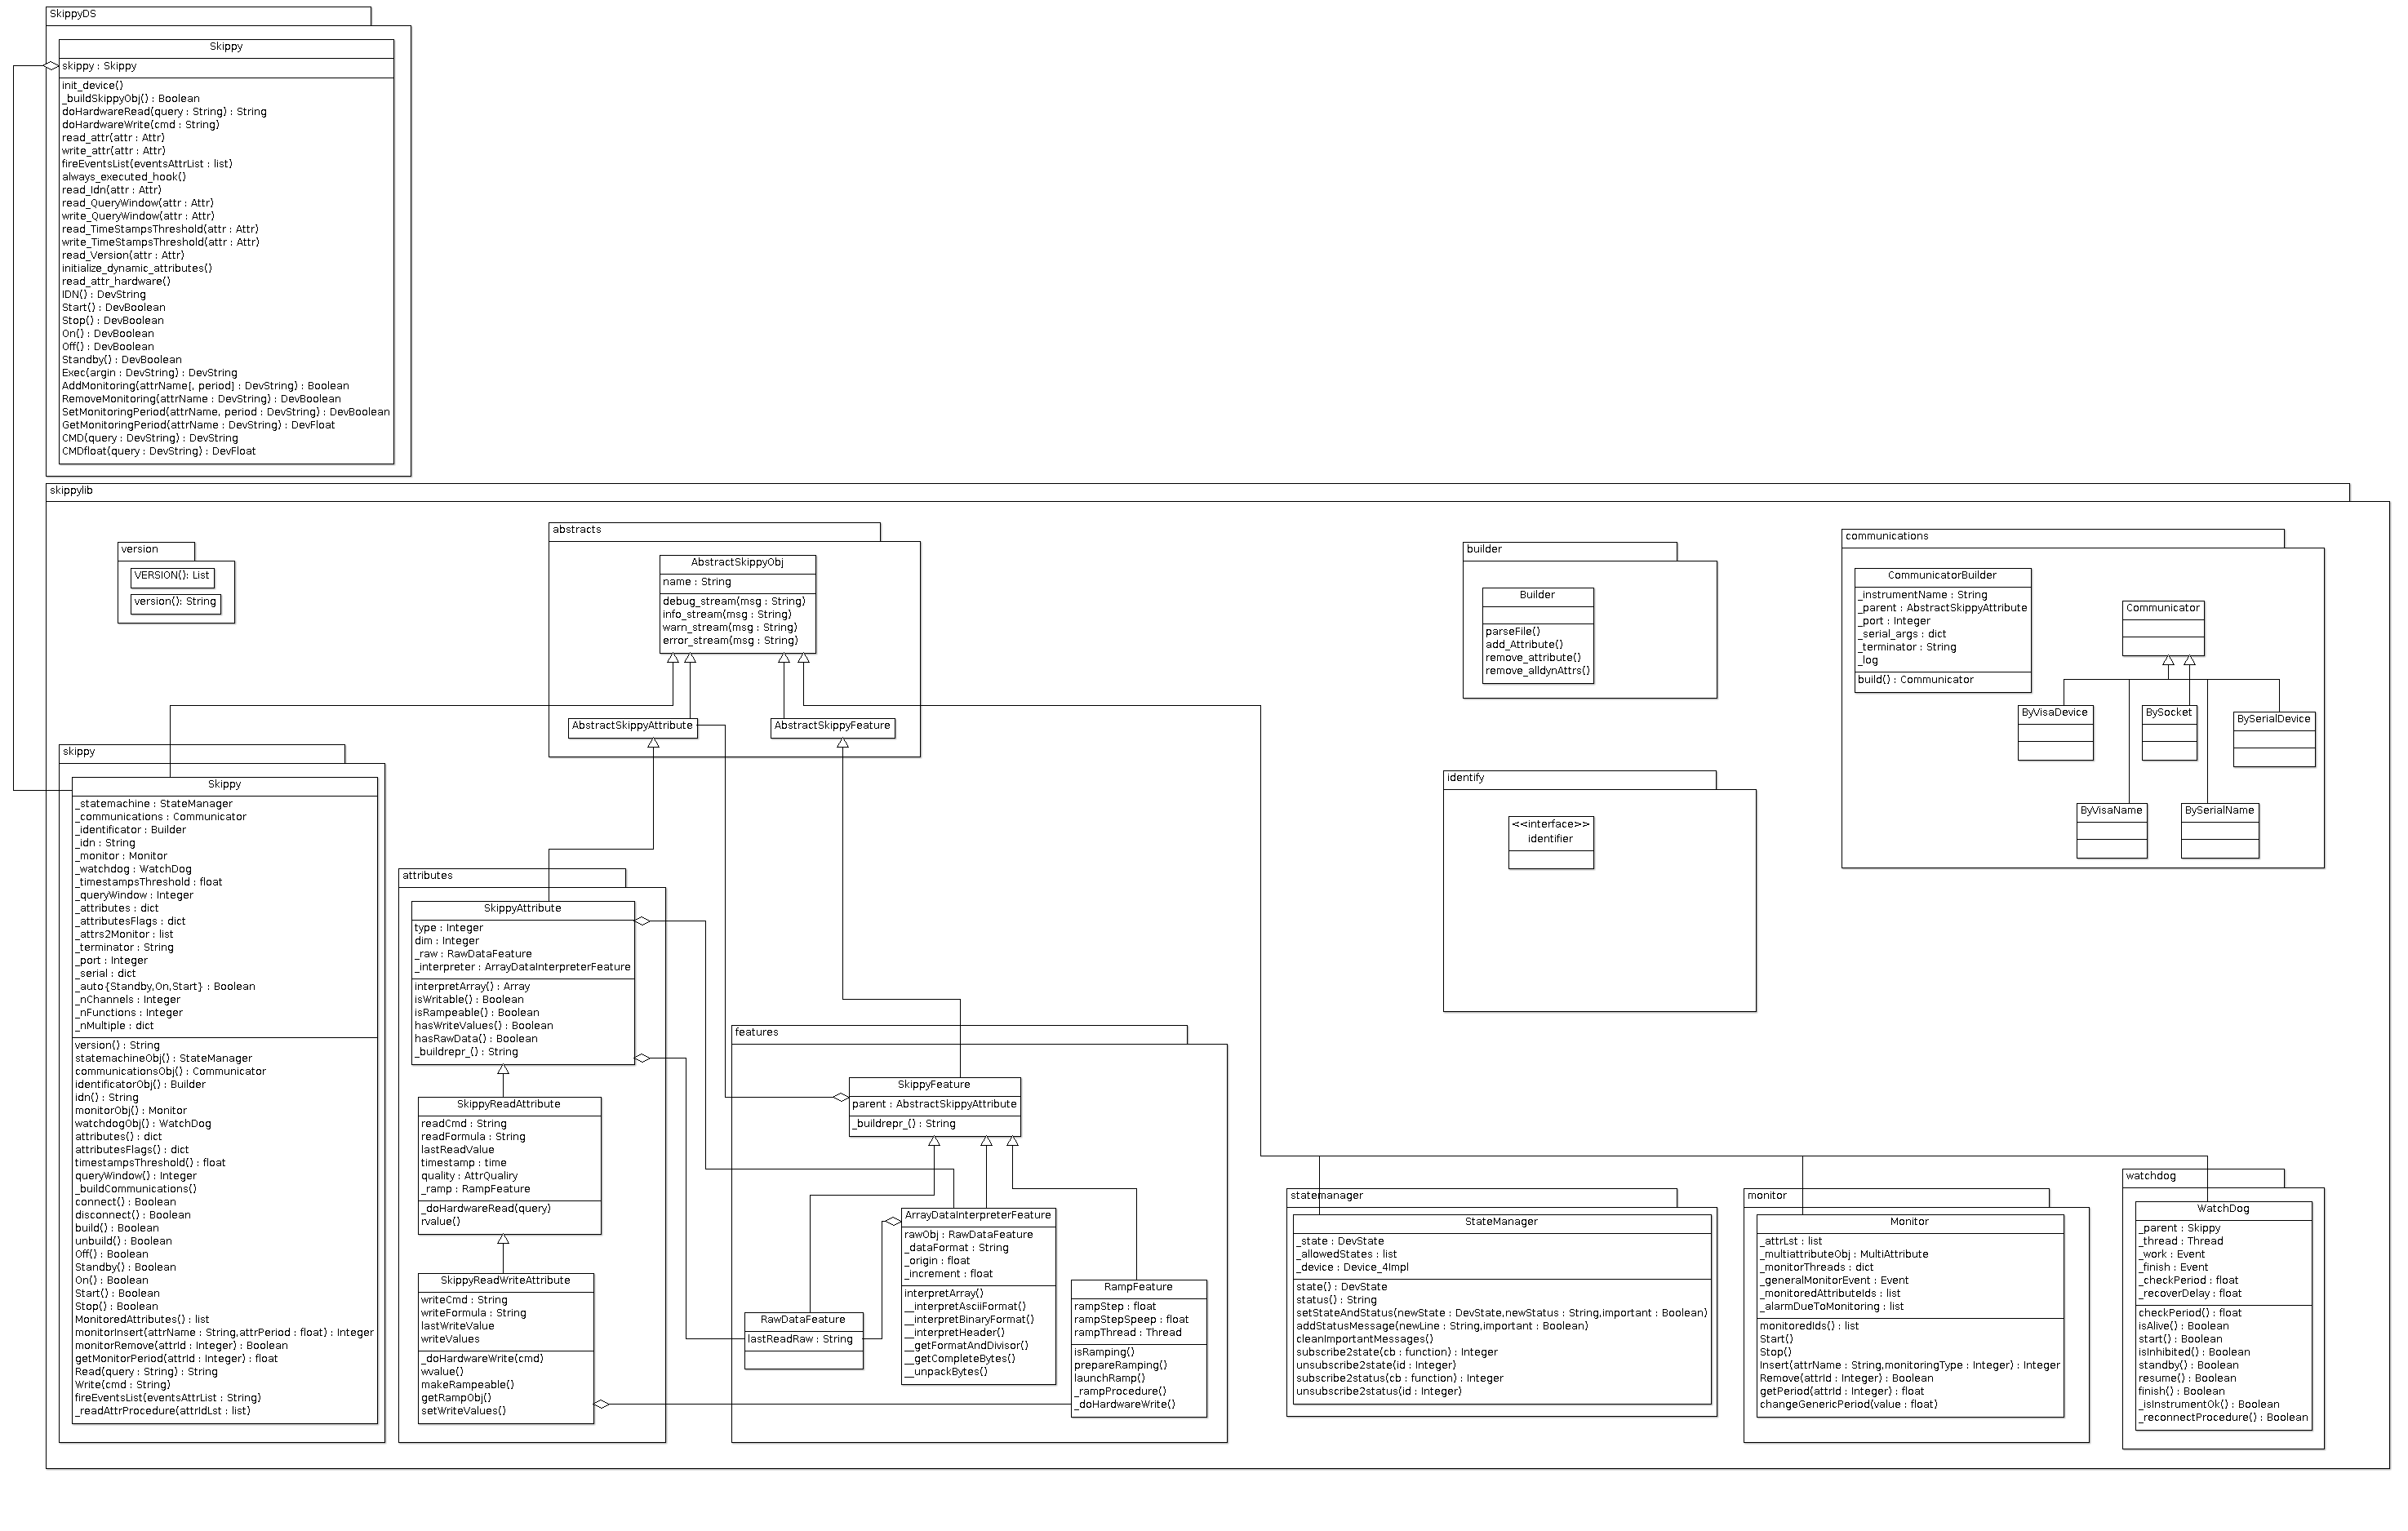
\includegraphics[width=\textwidth]{SkippyGeneralClassDiagram.png}
         \caption{Class diagram of the Skippy device.} \label{fig:classDiagram}
    }
\end{figure}

\section{Device features}\label{sec:devFeatures}

\subsection{Dynamic commands}\label{sec:dynCmds}

This feature is not yet implemented

\subsection{Dynamic attributes}\label{sec:dynAttrs}

Device is capable to dynamically build attributes based on the instrument identification (described in the the particular instruction set).
\begin{itemize}
    \item Supported Scalar and Spectrum (1 dimension arrays) attribute definition. Image (2 dimension arrays) are not currently developed, neither in the schedule because they are not needed by any of the current supported instruments. Although the device is prepared to sopport them if need be. (Perhaps the frequencies spectra in SpectrumAnalyser).
    \item The dynamic attributes build after the instrument identification can be Memorized if this has been configured this way in the file with the instruction set.
\end{itemize}

\subsection{Multiple requests per query}\label{sec:multiquery}

Multiple request of data to the instrument: As figure \ref{fig:groupedRequests} describes, when the device receives a request for reading to the instrument it can manage to cut those requests in subsets to avoid stress in the instrument. The communication itself supports a direct socket connection to the instrument and the use of the \emph{PyVisa} device as a bridge in the communication. 

\begin{figure}[h]
    \centering{
         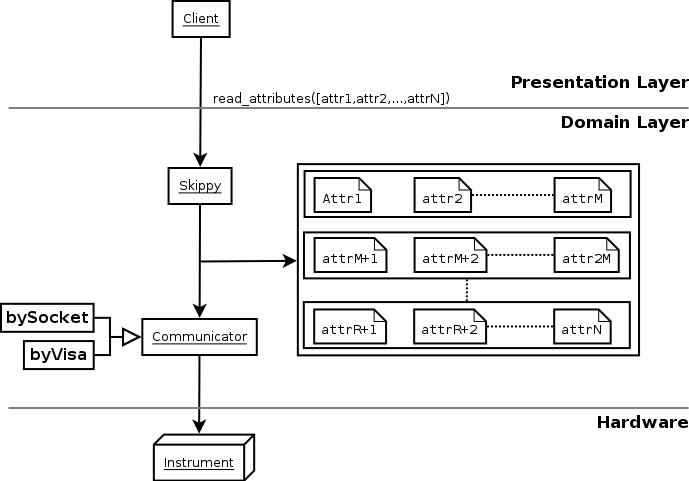
\includegraphics[width=0.75\textwidth]{groupedRequests.png}
         \caption{multiple request of readings to the instrument.} \label{fig:groupedRequests}
    }
\end{figure}

\subsection{Write attributes ramping}\label{sec:ramping}

Write process to some attributes would require a smooth ramp. As an example, to change the frequency in the \emph{RFGenerator}, the change would not be set directly (or the timing system will suffer). Then in the build process of an specific attribute with a certain flag of "movability" (name to be determined) two extra attributes, internals in the device, must be built also: a \texttt{Step} and a \texttt{StepSpeed}. On the write operation a thread is launched and every "StepSpeed" seconds change the value by the content in "Step" in the direction to the final setpoint. This was already implemented in \emph{PyRfSignalGenerator} Class. \fixme{This will require a refactoring in order to encapsulate the functionality in a \emph{responsible object}}.

\subsection{Monitoring values}\label{sec:monitor}

Monitor attributes. Having a property with a list of attributes, if they exist in the instrument definition, configure them in events and do a separated thread polling that will emit events on this attributes. This feature is different that setting up a "polling" from tango to the attribute because this fails to use the multiple reading.

\begin{itemize}
    \item In the definition of the attribute to be monitored, the \emph{MonitoredAttributes} property, using an specific notation (a ':' followed by a number of seconds) can set up an specific monitoring period for it in particular.
    \begin{itemize}
	\item When the monitoring is by the specific period, different attributes with the same period, should be read by the same monitor thread.
    \end{itemize}
    \item The use of the commands (\emph{add} and \emph{remove}) to setup this feature is recommended. Together with a set of commands to setup specific monitoring periods.
    \item When an attribute is monitored, a {\tt read\_attr()} returns the cached value (no hardware read).
\end{itemize}

\todo{Once this monitoring feature is available, other attributes not monitored that have reached some reading frequency, would be included in the monitoring loop (not emitting events) in order to reduce the load of the readings. The frequency reading should be monitored to notice when this has reduced over another threshold to avoid unnecessary readings.}

\fixme{When many attributes are being read, and not by {\tt read\_attributes([])}, prioritise. (This happens, for example, when opens the device with \emph{Atkpanel}) }

\subsection{Watchdog}\label{sec:watchdog}

\todo{Explain}

\section{Testing}\label{sec:testing}

\subsection{Scripts}

\todo{describe the \texttt{Testing} directory files and usage.}

\subsection{Known bugs}\label{sec:bugs}

\begin{itemize}
    \item \fixme{When all the monitored attributes are removed, the list ends inconsistent and dirty when newer attributes are added to this list.}
    \item \fixme{The timestamp of an attribute come from when it was read from the hardware. But in case of an \texttt{INVALID} value, it will point forever to when it has decay: this produces issues when a plot show this and other attributes with different time scale.}
    \item \fixme{The an instrument is powered off, if there is no attribute monitor the device will not see it until access the hardware. That is, request the \emph{state} before write will not update the information.}
    %\item \fixme{It have seen, when the read frequency is very fast, like read a waveform above $5Hz$, some exceptions that suggest a responses cross between spectrum and scalar. This is potentially critical, because is undetectable if it happens between scalars.}
    %\item \fixme{When a function is not defined (not when if off like a channel, this is like ask for a channel that doesn't exist physically), the device hangs due to an exception from the instrument and a very long time out.}
\end{itemize}

\end{document}
